\chapter{Study of Literature}

\textbf{Author: } 

\section{Different Approaches to the Problem}
Localising a robot in an unknown surrounding can be achieved by a multitude of different sensors. To name a few stereo cameras, LIDAR systems, ultrasonic sensors and time-of-flight cameras all measure the distance to the objects located around the robot. This data can then be used to gather information about the current location of the robot or aid navigation.

\section{Stereo Camera}
The challenge of sensing distances to various objects has been solved using stereo vision cameras. Computer stereo vision systems use two horizontally displaced cameras to take two images which then are both processed together to gather the information on the depth of the images. This process can be rather complicated as the distortions of the images have to be undone, before the two images can be projected onto a common plane, a disparity map can be created by comparing the two images and a 3d point cloud can be generated from this comparison. In most robotics applications this point cloud is then filtered in search of some object, which distance was sought-after.

\subsection{Distortion}
One of the distortions that have to be undone before the images can be processed any further is called barrel distortion. It occurs when the lens used by the camera has a higher magnification at the centre of the image than at the sides. This distortion can be visualized as seen in Figure~\ref{pic:methodology_stereoCamera_distortion_barrelDistortion}.

\begin{figure}[h!]
	\centering
	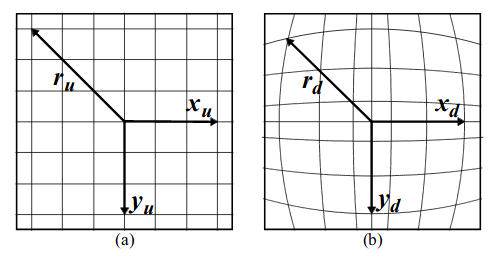
\includegraphics[width=4.5in]{img/methodology_stereoCamera_distortion_barrelDistortion.png}
	\caption{The left shows the original image composed of straight horizontal and vertical lines. On the right image the effect of the barrel distortion can be seen. The distortion causes the lines to curve toward the outside of the image, causing the lines to appear in a barrel like shape. [TODO: change image to own]}
	\label{pic:methodology_stereoCamera_distortion_barrelDistortion}
\end{figure}

Gribbon et.al. \footcite{Gribbon_Barrel_Distortion_Correction_Algorithm} propose equations, which calculate the pixel values in the undistorted image based on the pixel values in the distorted image.

In comparison to barrel distortion tangential distortion displaces points along the tangent of a circle placed at the centre of the image as seen in Figure~\ref{pic:methodology_stereoCamera_distortion_tangentialDistortion}.

\begin{figure}[h!]
	\centering
	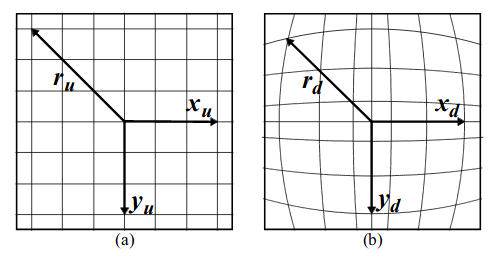
\includegraphics[width=2in]{img/methodology_stereoCamera_distortion_tangentialDistortion.png}
	\caption{A point $P$ is distorted along the tangent $t$ of a circle placed at the middle of the image $C$ with a radius $r$ to a point $P'$. Distortions of this form are called tangential distortions.}
	\label{pic:methodology_stereoCamera_distortion_tangentialDistortion}
\end{figure}

The radius of the circle in Figure~\ref{pic:methodology_stereoCamera_distortion_tangentialDistortion} is dependent on the point $P$. It can be calculated as the length between $P$ and $C$. The length of the vector $PP'$ is not uniform for all points and therefore depends on point $P$.

\subsection{Image Rectification}
Image Rectification projects multiple images taken from different points of view onto a common plane. 

\begin{figure}[h!]
	\centering
	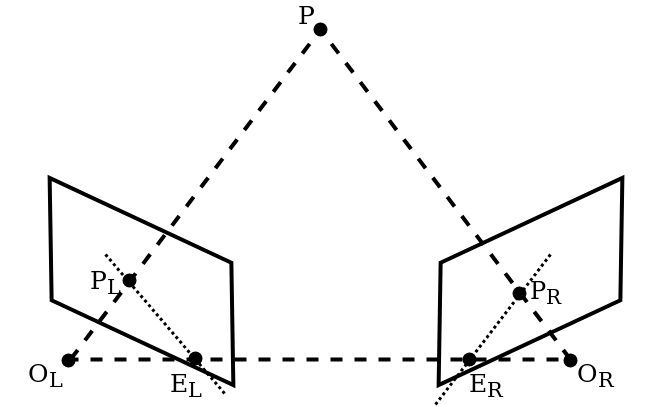
\includegraphics[width=4in]{img/methodology_stereoCamera_imageRectification.png}
	\caption{Two images containing some point $P$ are taken from the two points $O_L$ and $O_R$. Point $P$ is projected in the image planes as points $P_L$ and $P_R$. $E_L$ and $E_R$ depict the epipoles.}
	\label{pic:methodology_stereoCamera_imageRectification}
\end{figure}

Chan et. al. propose an image rectification algorithm \footcite{Chen_New_Image_Rectification_Algorithm}, which follows the following sequence of events:

\begin{enumerate}
	\item At least seven matching points visible on both images are found.
	\item The fundamental matrix (as well as the epipoles) are estimated.
	\item The common region is identified (using epipolar geometry constraints).
	\item The epipolar line is transferred and the Bresenham algorithm\footcite{Bresenham_Linear_Algorithm_For_Incremental_Digital_Display_Of_Circular_Arcs} is used to extract pixel values.
	\item The rectified image is resampled.
\end{enumerate}

\subsection{Disparity Map}
A disparity map represents the depth of an image. It can be calculated by comparing the position of pixels in two images made for example by a stereo camera. Objects, that are closer, have a larger difference in their relative position on the two image, than objects that are farther away.

One approach, which focuses not only on the quality of the disparity, but also on the time needed to compute the result, is described in the work of Mühlmann et.al\footcite{Muehlmann_Calculating_Dense_Disparity_Maps_from_Color_Stereo_Images}.

\subsection{3D Point Cloud}
To generate a 3D point cloud out of the disparity map a two dimensional image has to be converted into a three dimensional space. This is done by extracting the information about the depth for each pixel from the disparity map. In our use case the resulting 3d point cloud then has to be filtered in search of the object, which distance to was sought after.

\section{LIDAR}
A lidar is a sensor that can be used to gather information about the environment. The sensor sends out light in a particular direction. Then the time needed for the light to return to the lidar is measured and the distance is calculated from that. By sending and receiving the light from multiple different directions data points from the entire two or three dimensional surrounding can be detected.

One example of a use case for a lidar sensor is demonstrated in the paper on Lidar-based teach-and-repeat of mobile robot trajectores of Spunk et al.\footcite{Sprunk_Lidar-based_teach-and-repeat_of_mobile_robot_trajectories}. The objective of their work is to teach a robot some trajectory by demonstration and then have the robot repeat the same trajectory as closely as possible. Their use of a lidar sensor enables them to follow the given trajectory with an accuracy of a few millimetres.

\section{Structure from Motion}
Similar to a stereo camera structure from motion estimates the three dimensional structure of the surrounding from the information of two dimensional images. The difference lies in the number of images typically used. While stereo cameras use two images, structure from motion commonly takes more images to reconstruct the three dimensional scene.

Structure from Motion can be used whenever it is necessary to take multiple images. This can be the case when one image can not include all of the relevant data that should be processed, for example when modelling terrain.

\section{Depth Maps from Structured Light}
By taking an image of an specially illuminated scene the structured light approach is able to calculate a depth map. Scharstein et al. present an approach that constructs high accuracy depth maps without the need to calibrate the light sources. \footcite{Scharstein_High-accuracy_stereo_depth_maps_using_structured_light} So get information on specific distances to objects additional data, such as a different sensor measuring the distance to some (other) point in the image, is needed.

\section{Human Depth Perception}
In medicine depth perception defined as the ability to see three dimensional space and judge distance accurately. Humans achieve depth perception by combining information from multiple depth cues. A depth cue is a feature of the environment or the person itself, that can be used to judge distance to objects. Depth cues can be classified in either of two categories: binocular and monocular, where binocular depth cues require two eyes and monocular only require one eye to work.

Which depth cue is used by humans in which situation was researched by Schrater et al. \footcite{Schrater_How_optimal_depth_cue_integration_depends_on_the_task}.

\begin{table}[h!]
	\begin{tabularx}{\textwidth}{|l|X|}
		\hline
		\multicolumn{2}{|l|}{\textbf{binocular depth cues}} \\
		\hline
		retinal disparity & Because the two eyes of a human person are separated by a few centimetres each eye perceives the environment from a slightly different point of view. These differences in the position of objects on the retina can be calculated as described by Cormack et al. \footcite{Cormack_The_computation_of_retinal_disparity}.\\
		\hline
		convergence & To focus on objects farther away the eyes have to be less crossed than when focusing on near objects. It is debatable whether the information on how crossed the eyes look is used by all humans to gather information on depth. Richards et al. designed a test and found that approximately two thirds of the population can use convergence as a depth cue. \footcite{Richards_Convergence_as_a_cue_to_depth} \\
		\hline
	\end{tabularx}
	\label{tab:study_of_literature_binocular_depth_cues}
	\caption{A short overview of different binocular depth cues used by humans to see three dimensional space and judge distance.}
\end{table}

\begin{table}[h!]
	\begin{tabularx}{\textwidth}{|l|X|}
		\hline
		\multicolumn{2}{|l|}{\textbf{monocular depth cues}} \\
		\hline
		accommodation & As the eye focusses on an object the lens changes its thickness. The difference in thickness may be used to determine distance similar to convergence.
		\\
		\hline
		light and shadow & The position on which a shadow of an object falls can give information on its position in three dimensional space. This phenomenon can be observed in Fig.~\ref{pic:study_of_literature_depth_perception_two_shperes}.
		\\
		\hline
	\end{tabularx}
	\label{tab:study_of_literature_monocular_depth_cues1}
	\caption{A short overview of different monocular depth cues used by humans to see three dimensional space and judge distance.}
\end{table}


\begin{table}[h!]
	\begin{tabularx}{\textwidth}{|l|X|}
		\hline
		\multicolumn{2}{|l|}{\textbf{monocular depth cues}} \\
		\hline
		linear perspective & Parallel lines in the environment, such as railroad tracks, appear to converge in one point. Therefore when shown an image containing converging lines, such as Fig.~\ref{pic:study_of_literature_depth_perception_two_shperes}, the two dimensional picture conveys depth. Yonas et al. performed an experiment, showing at what point in their life infants develop the ability to use linear perspective.  \footcite{Yonas_Infants_distance_perception_from_linear_perspective_and_texture_gradients}
		\\
		\hline
		texture gradients & According to Ganong \footcite{Ganong_Review_of_Medical_Physiology} the retina takes up two thirds of the inner side of the eyeball. It is covered with cone cells, which are able to detect light. Since the retina only contains a finite number of cone cells, which are placed some distance apart, the eye can only detect its surrounding at a limited resolution. Therefore objects farther away seem smoother as fine details can not be detected as easily.
		\\
		\hline
		overlap & Overlapping is a depth cue humans develop early in their life. It is described as getting information on the order of objects sorted by their distance by looking at the way objects hide parts of other objects. Hagen tested sensitivity of overlapping as a depth cue in three, five and seven year old children and found that all where able to perceive depth based on this information. \footcite{Hagen_Development_of_ability_to_perceive_and_produce_pictorial_depth_cue_of_overlapping}
		\\
		\hline
		aerial perspective & Very far distanced objects may appear hazy in certain weather conditions. The distance to these objects can be estimated by the haziness at which they appear.
		\\
		\hline
		relative motion & When the observer changes position the position at which objects are sensed change. The distance the objects change position in the eyes of the observer can be used to determine the how far it is away. Closer objects move further while farther objects move less when the observer moves. This depth cue is called relative motion or motion parallax. According to Rogers et al. humans can reliably reconstruct distance from relative motion alone. \footcite{Rogers_Motion_parallax_as_an_independent_cue_for_depth_perception}.
		\\
		\hline
	\end{tabularx}
	\label{tab:study_of_literature_monocular_depth_cues2}
	\caption{A short overview of different monocular depth cues used by humans to see three dimensional space and judge distance.}
\end{table}

\begin{figure}[h!]
	\centering
	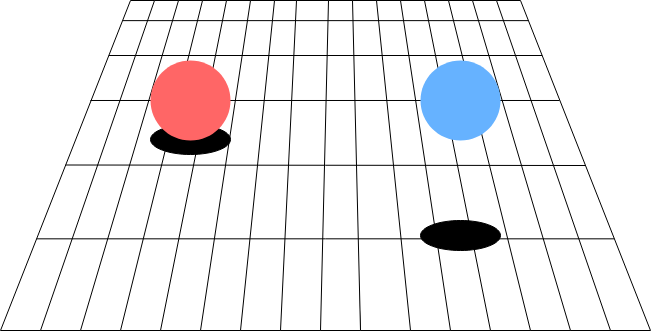
\includegraphics[width=4in]{img/study_of_literature_depth_perception_two_shperes.png}
	\caption{A two dimensional image conveying depth using linear perspective. The blue sphere seems closer than the red one, because of its shadow. Meanwhile the red sphere appears bigger as it is farther away and has the same relative size in the two dimensional image.}
	\label{pic:study_of_literature_depth_perception_two_shperes}
\end{figure}

\subsection{Depth Sensation}
Since it is not clear to what extent animals and infants can determine depth and sense their three dimensional environment the term depth perception is not used. It has been shown however that at least some animals can sense depth and therefore experience depth sensation.

One experiment which tests depth sensation is called visual cliff. \footcite{Gibson_The_visual_cliff} The task of the test subjects is to identify a sharp drop over which they must move to reach a desired destination. The setup of the experiment can be found in Fig.~\ref{pic:study_of_literature_depth_perception_depth_sensation_visual_cliff}. It has been shown that infants along with all tested animals stop as soon as they have reached the cliff. Therefore they must experience some sort of depth sensation.

\begin{figure}[h!]
	\centering
	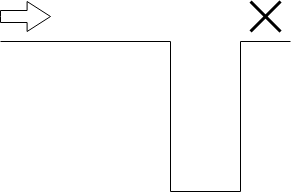
\includegraphics[width=3in]{img/study_of_literature_depth_perception_depth_sensation_visual_cliff.png}
	\caption{Setup of the visual cliff experiment. The arrow marks the starting point of the test subject. At the position of the X a desirable object is placed. Therefore the test subject starts moving toward the goal. If the subject has depth sensation it will stop before the cliff, while subjects without depth sensation won't be able to detect the cliff and therefore won't stop.}
	\label{pic:study_of_literature_depth_perception_depth_sensation_visual_cliff}
\end{figure}

\filbreak